\section[Overall Description]{\hyperlink{toc}{Overall Description}}

\subsection[Product Perspective]{\hyperlink{toc}{Product Perspective}}
	Thanks to the general introduction and the scope definition of the system from the previous sections, we are now able to look at our system first from the outside and then from the inside. To deal with this description we are going to see the external interfaces of the system and then the definition of the model's structure in order to interact with them; at the end of the section \textbf{state diagrams} are used to emphasize the dynamic behavior of the most critical classes.
	\subsubsection[System Interfaces]{\hyperlink{toc}{System Interfaces}}
		\label{sec:systemInterfaces}
		SafeStreets offers an interface to its customers to provide them its basic and advanced functionalities. All the data needed to authenticate the users will be managed inside the system as well as the information related to the violations in order to be mined and crossed whenever needed.\\
		
		To accomplish the \hyperref[sec:goals]{\textcolor{blue}{goals}} stated in the \hyperref[sec:introduction]{\textcolor{blue}{introduction}} the application needs also to interact with three main external interfaces as reported in the following picture (\autoref{fig:systemInterfaces}).  
		\vspace{0,3cm}
		
		\begin{figure}[h]
			\centering
			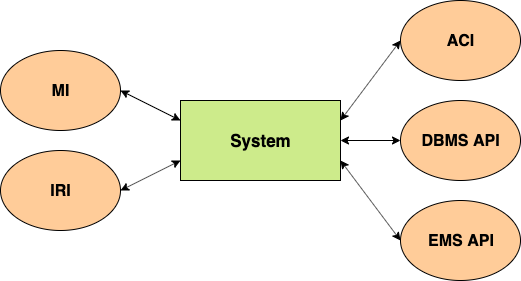
\includegraphics[scale=0.5]{/diagrams/externalInterfaces.png}
			\caption{\label{fig:systemInterfaces}System Interfaces}
		\end{figure}
		
		Two different kinds of interfaces are distinguished in the picture above:
		\begin{itemize}
			\item \textbf{Left hand side:} interfaces that provide functions (by means of APIs) for the system to perform internal operations. 
			
			In particular:
			\begin{itemize}
				\item \textsc{IRI} is used to process the image received from a violation. Whenever a violation is reported the system tries to recognize two distinct things from the picture helped by the additional data provided:
				\begin{itemize}
					\item \textbf{Plate:} the recognition of the plate's number is important to identify the vehicle by checking if it coincides with the one inserted or to add this information when missing. In both the cases when the number can not be identified the violation will be processed without it.
					\item \textbf{Type of vehicle:} is also very important to be recognized as the statistics can also be integrated with this filter. The vehicle will be reported without any type in case the process fails to find one, but we can assume that a shape recognition will be easily carried out by today's functionalities.
				\end{itemize} 
				\item \textsc{MI} is used to handle the geographical issues. The system needs to:
				\begin{itemize}
					\item \textbf{Retrieve} the name of the street where the violation occurred by using the provided position
					\item \textbf{Highlight} the safety of the streets and of municipality's areas
				\end{itemize}
			\end{itemize}
			\item \textbf{Right hand side:} interfaces that enable the system to send and receive data to the authorities. 
			
			In particular when:
			\begin{itemize}
				\item The reported violation has been accepted by the system and enriched with the metadata that can be useful for the authority. In this case the correct information is sent to the authority interested in the area that contains the related position.
				\item The municipality provides information about the accidents that occur in its area. Received data is crossed by the system to determine the safety of its streets. Thanks to this additional operation the application is also able to determine the best interventions for unsafe areas and suggest them to its users.
			\end{itemize}
		\end{itemize}
	
	\subsubsection[Model Structure]{\hyperlink{toc}{Model Structure}}
	The static analysis now continues to define the internal structure of the system, in particular with a high-level class diagram that shows the most important objects and their relations in order to achieve the \hyperref[sec:goals]{\textcolor{blue}{goals}}.\\
	
	The main objects in the UML diagram (\autoref{fig:classDiagram}) are:
	\begin{itemize}
		\item \textbf{Customer:} the system has to track two types of users. The distinction, in fact, is fundamental to recognize the municipality providing accident's data but also to give a different level of visibility to the information asked by a request.
		
		\item \textbf{User:} identifies a citizen with all the data he provides in its registration. Users are the clients of the application that report parking violations and look for \textbf{general} statistics related both to the frequency of parking violations in a street or to the safety of an area and its related suggested intervention.
		
		\item \textbf{Authority:} identifies the authority/municipality with all the data related to its recognition. Authorities are the clients of the application that receive the reported violations by the users but they also: ask for \textbf{specific} statistics and provide data about the accidents (crossed by the system).
		
		\item \textbf{Registration:} is used to authenticate the customer in order to perform actions he can only do recognized as a user or an authority.
		
		\item \textbf{Violation:} represents a general traffic violation. This class is thought to be used in a future extension of the system in case more violations are going to be considered.
		
		\item \textbf{ParkingViolation:} is the result of a notification provided by a user. In this way the application considers all the possible information that is filled whenever an infraction is reported. As we see in the UML diagram the class contains: multiple images for an  improved help to both the image recognition algorithm and the authorities; the position retrieved by the GPS (used to find the name of the street); the plate's number and all other metadata.
		
		\item \textbf{Accident:} will be used to store the data received by the municipality. No more specific description can be given here because only when interfacing with the municipality we will be able to know how the data has to be managed.
		
		\item \textbf{Position:} stores the coordinates of where the parking violation occurred. The position of each accident will be used to retrieve the street thanks to the functionalities provided by the MI and thus obtain statistics of each street and area.
		
		\item \textbf{Street:} is one of the most important object to be managed. Each recognized street will be added to the system to achieve its basic and advanced functionalities. A street considers also how many infractions happened in it; this is thought to simplify the very computing mining and crossing algorithms.
		
		\item \textbf{Area:} is another important object, in particular for the advanced functionality. An area contains the streets relative to its limits and is managed by the municipality that will receive all the violations reported in it. Areas are also critical for the safety they will encounter; to underline this we have defined an only method in the diagram (getSafety) that will be used later to define the related \textbf{state diagram}.
		
		\item \textbf{Vehicle:} vehicles are identified by the image recognition algorithm in order to provide additional information to the filter.
		 
		\item \textbf{Car:} are expected to be the most reported type of vehicles because of their dimensions and utilization (typically identified by the plate).
		
		\item \textbf{Motorcycle:} should be also considered as "critical" vehicles. The system has to care of particular areas where lots of motorcycles happen to be all parked in the wrong way and in uncomfortable spots.
		
		\item \textbf{Bicycle:} our system is supposed to deal also with bicycles. Obviously it will be much more difficult for the authorities to retrieve their owners but they can be used by the application to suggest possible interventions in the areas where they happen to be definitely cumbersome.
		
		\item \textbf{Request:} is the general class representing the interaction of a user with the system whenever statistics about the frequency, safety or suggestion is asked by the customer. In order to answer with the correct data it will be important to retrieve the user who sends the request to provide him the right visibility.
		
		\item \textbf{BasicRequest:} is the request that deals with the basic functionality. Thanks to it the application will be able to capture the filters selected by the user and answer correctly.
		
		\item \textbf{AdvancedRequest:} is the request that deals with the advanced functionality. Thanks to it the application will be able to capture the requirements of the customer, that in this case can be: the safety of a municipality's area or the suggestion for a possible intervention.
	\end{itemize}
	
	\begin{figure}[h!]
		\centering
		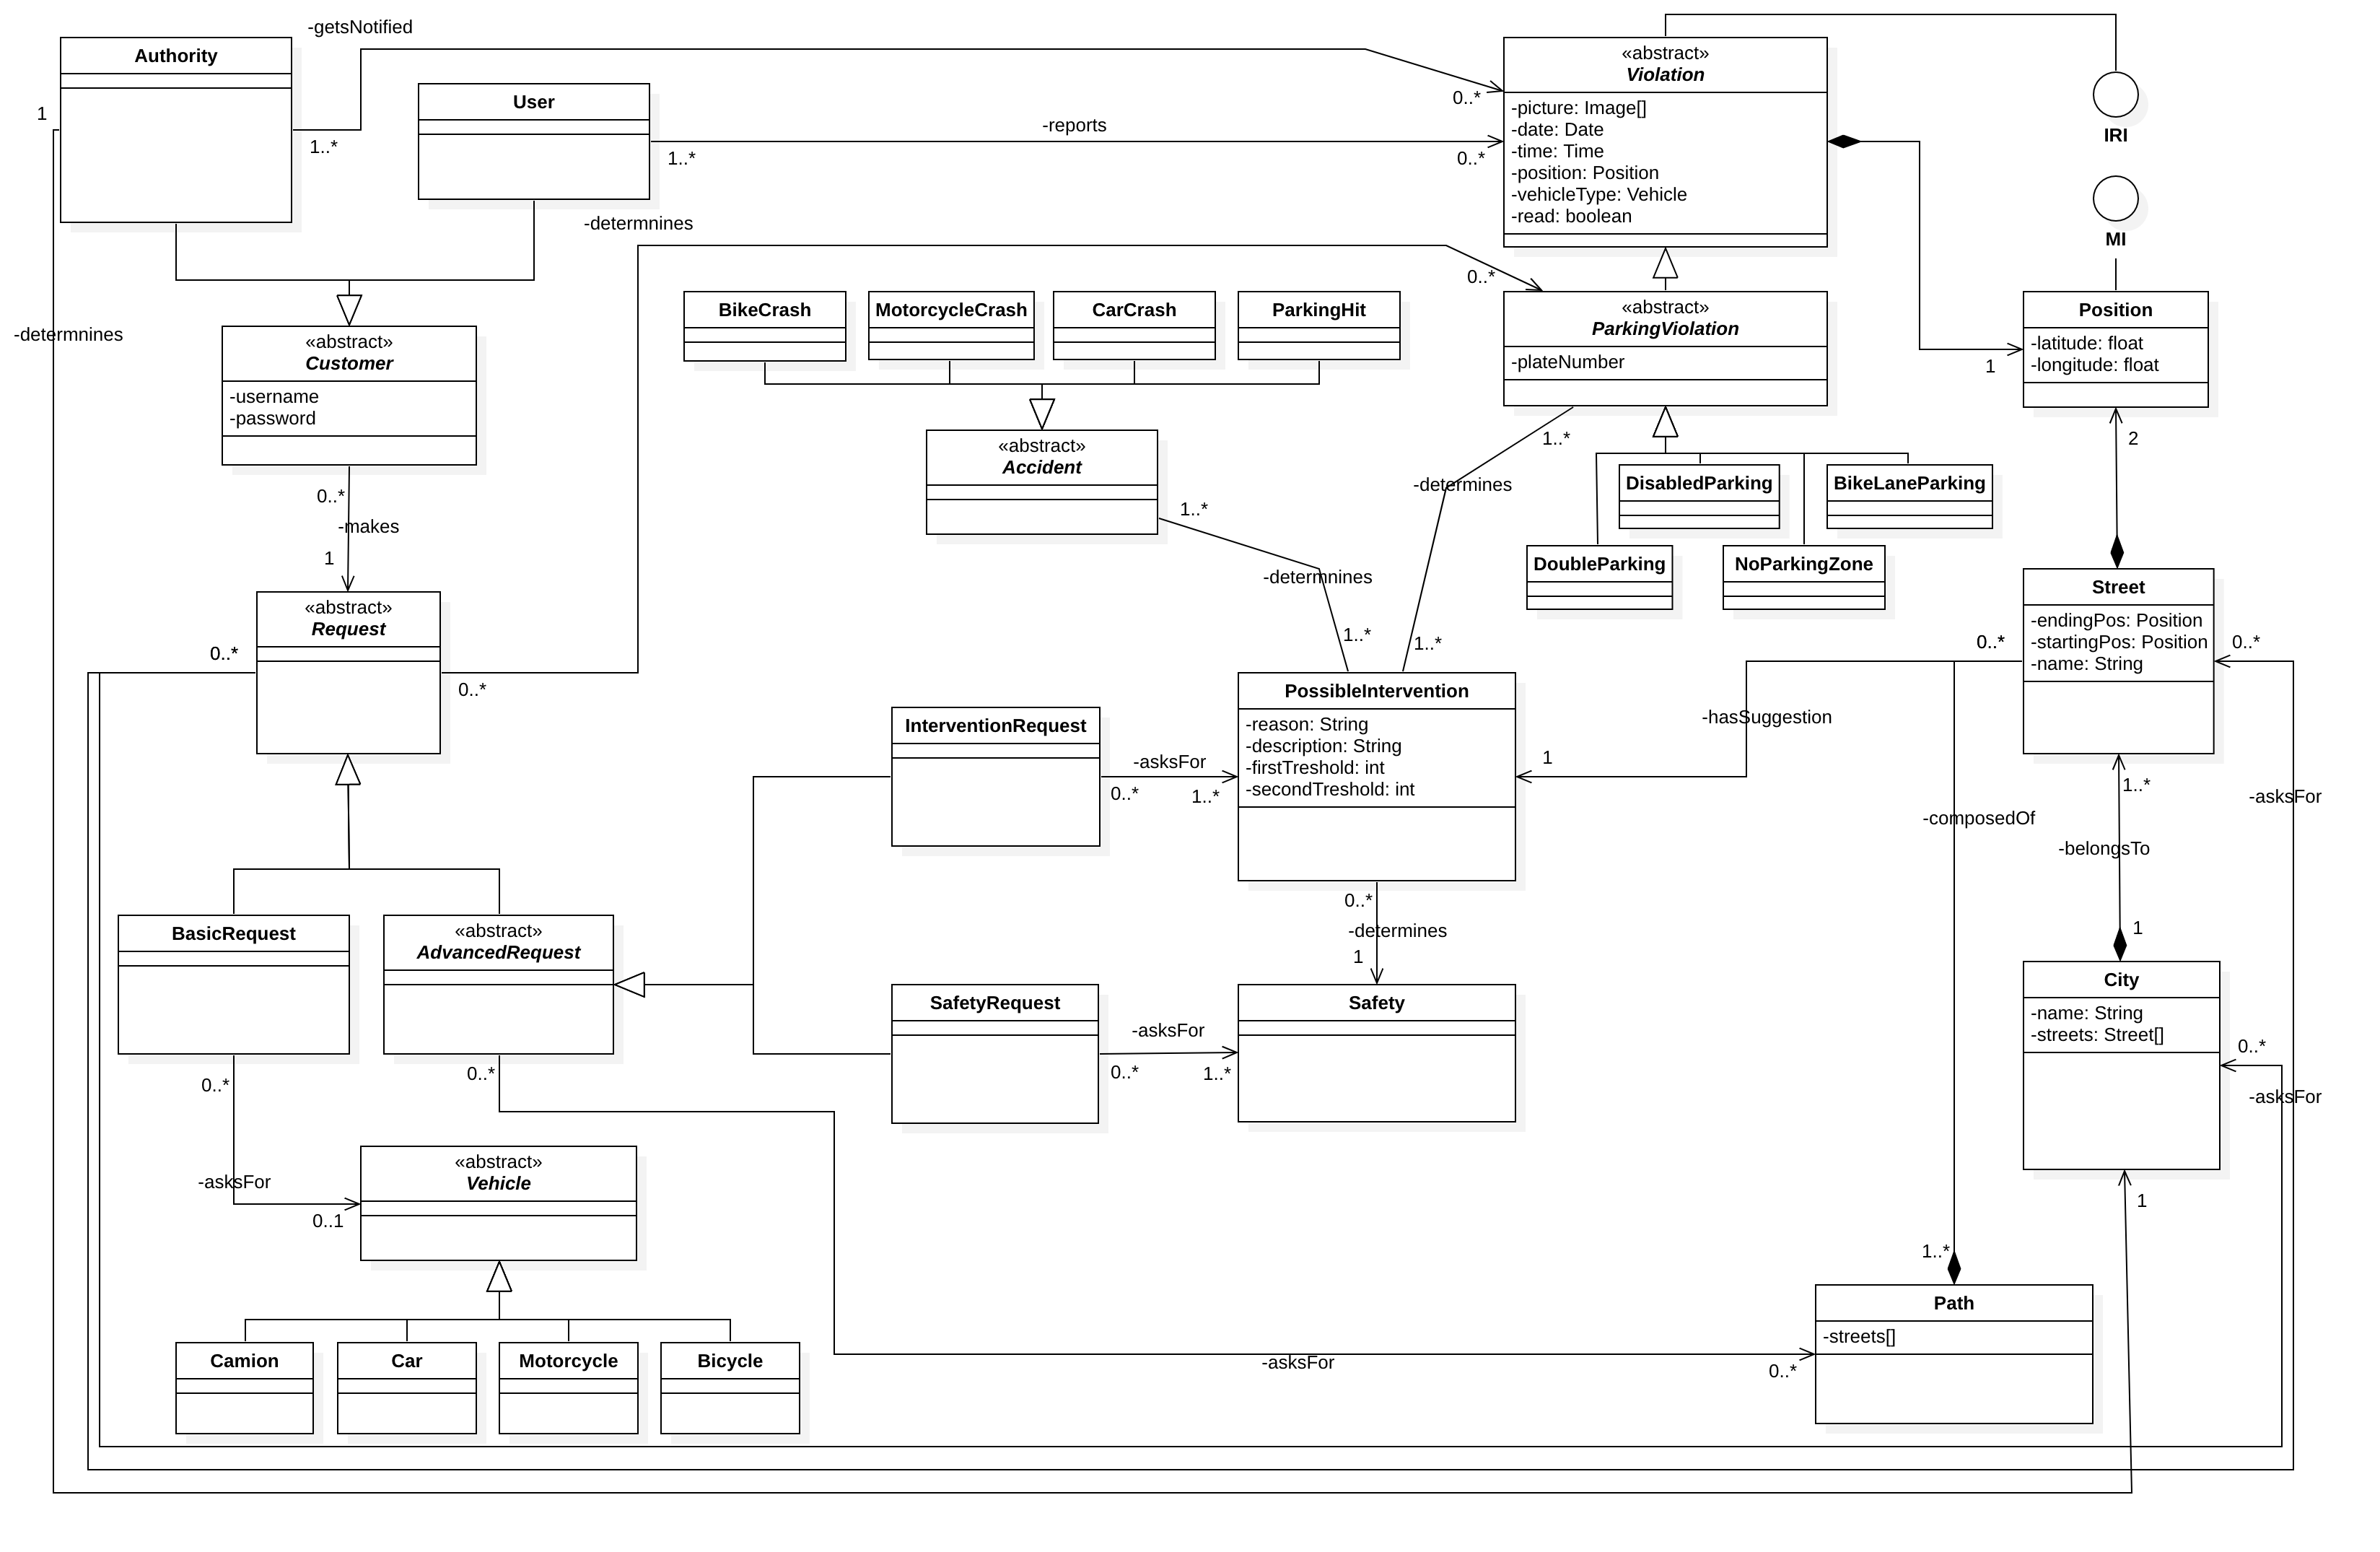
\includegraphics[width=\paperwidth - 1cm, angle=90]{/diagrams/classDiagramModel.png}
		\caption{\label{fig:classDiagram}High-level model structure}
	\end{figure}

	\FloatBarrier
	
	\subsubsection[State Diagrams]{\hyperlink{toc}{State Diagrams}}
	Considering now the main functionalities of the system, it is important to highlight the events that make its objects move from one state to another. State diagrams are used to describe the most critical aspects of the objects previously described in the UML diagram (\autoref{fig:classDiagram}).
	
	\paragraph{Notification}
		Beginning with the notification of a parking violation it is important to remember that each infraction will be refused by the system i.i.f inconsistency is found; for example multiple images representing different types of vehicles.
		The diagram (\autoref{fig:notifyState}) starts when a violation is received in the \textit{unprocessed} state. First the system needs to check the consistency of the data received in order to accept or reject the violation. If the message is \textit{rejected} the notification diagram ends, otherwise the \textit{accepted} violation needs some more checks before it can be stored in the system. Second another check is used to understand if the infraction lacks of some important fields to be stored that however the application should be able to retrieve easily thanks to the functionalities provided by the external interfaces. Then, if the message is \textit{complete} it is ready to be enriched with other metadata (the name of the street retrieved by the GPS position), otherwise it is completed with missing information and then the \textit{ready} state is reached too. Lastly the information about the parking violation is \textit{stored}in the system, \textit{sent}to the authority and the notification diagram ends.
		
		\vspace{0.3cm}
		\begin{figure}[h]
			\centering
			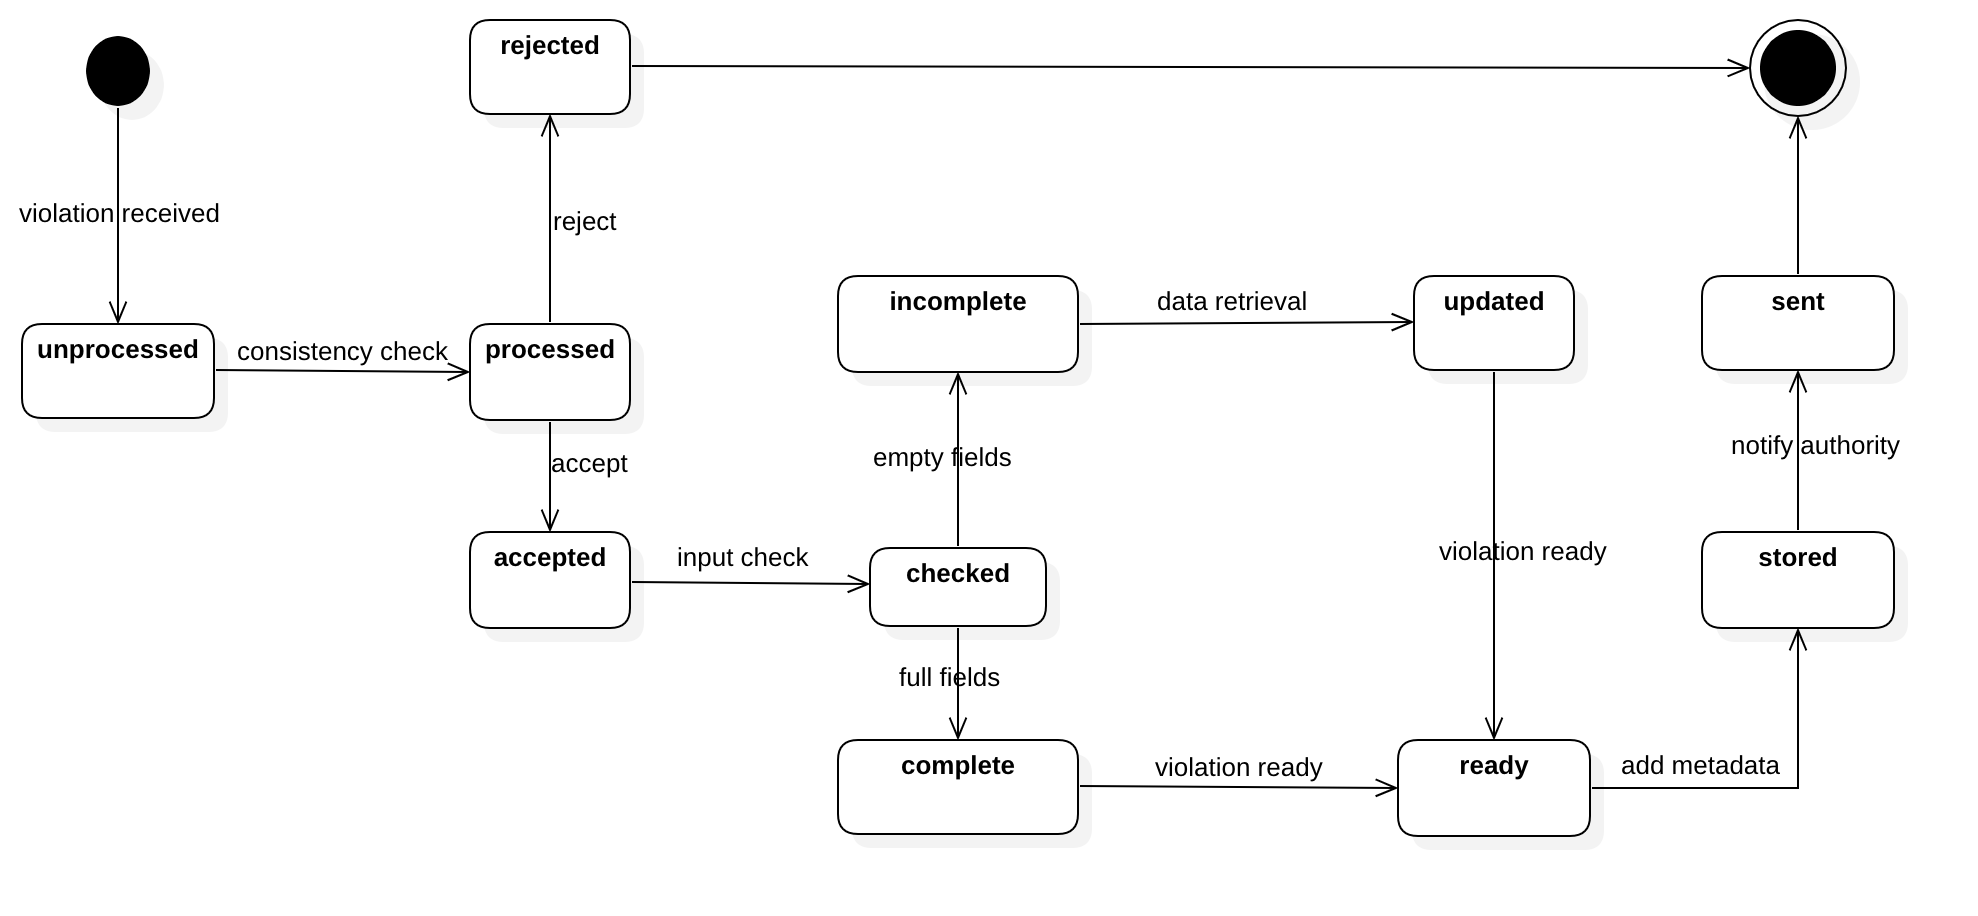
\includegraphics[scale=0.18]{/diagrams/notifyStateDiagram.png}
			\caption{\label{fig:notifyState}Notification state diagram}
		\end{figure}
	
	\paragraph{Request}
		Statistics retrieval is another critical functionality that needs a state diagram in order to define how the information asked is provided with different levels of visibility depending on the role of the customer.
		The diagram (\autoref{fig:requestState}) represents both different kinds of requests a customer can do, in fact it is used to highlight the different visibility of the answered information rather than the difference between the requests. Whenever a query is received, the system has first to retrieve the data that is required thanks to the filters provided by the customer. After the information is found in the \textit{processed} state, the application needs to recognize the user in order to provide him the data with the level of visibility devoted to him. If the request comes from a user its data is filtered and once ready (\textit{user data} state), sent back to the user; symmetrically happens for the authority who will receive the least aggregate information possible. 
		
		\vspace{0.3cm}
		\begin{figure}[h]
			\centering
			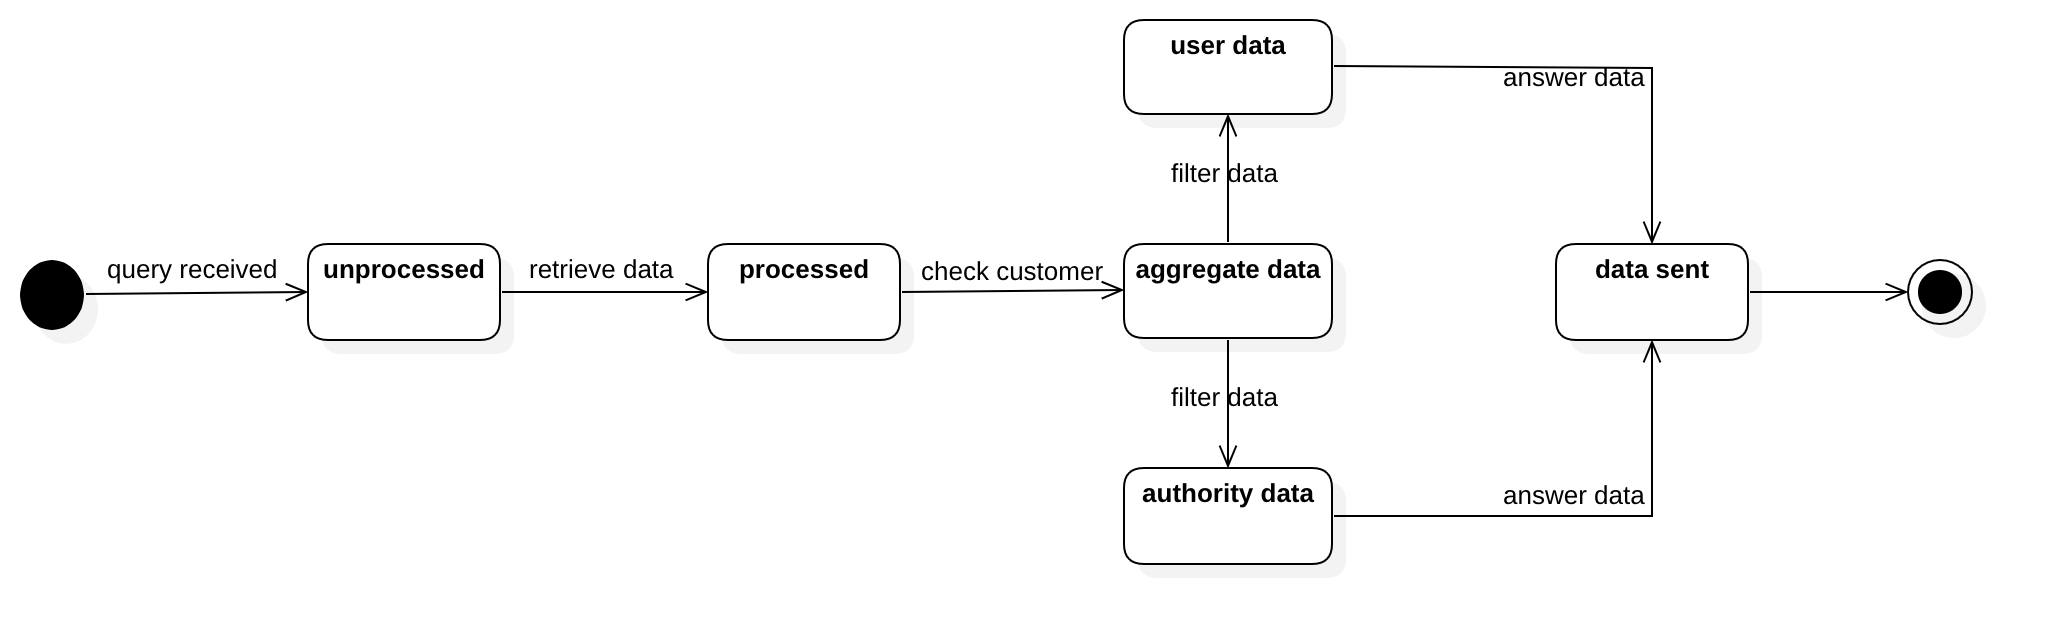
\includegraphics[scale=0.18]{/diagrams/requestStateDiagram.png}
			\caption{\label{fig:requestState}Request for data state diagram}
		\end{figure}
	
	\paragraph{Safety}
		The last state diagram is used to highlight how the system is able to determine the safety of a street and update its state whenever new violations occur or new accidents data is provided by the municipality. 
		The diagram (\autoref{fig:safetyState}) shows how the safety of a street evolves in the time. The system is able to cross its own data with the one provided by the municipality to establish the safety of an area that will be evaluated thanks to some tresholds. At the beginning an area is considered \textit{safe} (and highlighted with the GREEN color) because no parking violation are stored and no cross can be performed. Once parking violations start to occur the application is able to keep track of their frequency and, thanks to the accidents information, will determine if the area has to be considered less safe than before or not. In this way once exceeded the safe treshold it will be considered \textit{half safe} (highlighted in YELLOW) and the same for the last state that represents an \textit{unsafe} area (highlighted in RED). Obviously the system has also to consider when an area enhances its safety; this will happen whenever one of the tresholds is not reached anymore. 
		
		\vspace{0.3cm}
		\begin{figure}[h]
			\centering
			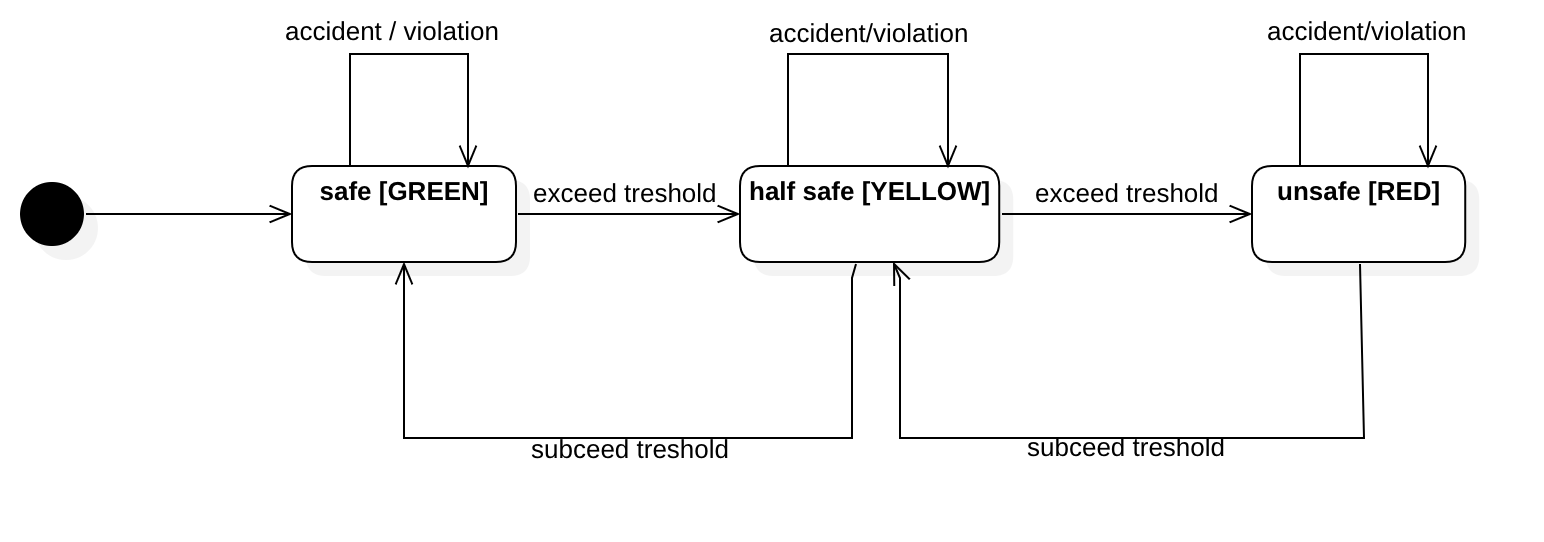
\includegraphics[scale=0.23]{/diagrams/safetyStateDiagram.png}
			\caption{\label{fig:safetyState}Area safety state diagram}
		\end{figure}   

\subsection[Product Functions]{\hyperlink{toc}{Product Functions}}

\subsection[User Characteristics]{\hyperlink{toc}{User Characteristics}}

\subsection[Domain Assumptions]{\hyperlink{toc}{Domain Assumptions}}

\subsection[The World and the Machine]{\hyperlink{toc}{The World and the Machine}}